\documentclass[trans]{beamer}
\usetheme{Pittsburgh}
% \usetheme{Montpellier}
% \usetheme{Hannover}
% \usetheme{Warsaw}

% \mode<presentation> { \usetheme{Warsaw} %other themes 
%   %Warsaw presentation Pittsburgh print
%   \setbeamercovered{transparent}
% }

\usepackage[spanish]{babel}
\usepackage[latin1]{inputenc}
\usepackage{times}
\usepackage[T1]{fontenc}
\usepackage{pifont}
% \usepackage[pdftex]{hyperref}
\title[Introducci\'on informal a Matlab y Octave] 
{Introducci\'on informal a Matlab y Octave}


\author[Guillem Borrell Nogueras]
{Guillem Borrell Nogueras\inst{1}\\
\texttt{guillemborrell@gmail.com}\\
\texttt{http://torroja.dmt.upm.es:9673/Guillem\_Site/}}
\institute[Delegaci\'on de alumnos] 
{
  \inst{1}%
  Delegaci\'on de alumnos\\
  ETS Ingenieros Aeron\'auticos\\
  Universidad Polit\'ecnica de Madrid
}

\date[Introducci\'on a Matlab]
{Curso 2005/2006}
\subject{Matlab}

\AtBeginSubsection[]
{
  \begin{frame}<beamer>
    \frametitle{\'Indice}
    \tableofcontents[currentsection,currentsubsection]
  \end{frame}
}

\begin{document}

\begin{frame}
  \titlepage
\end{frame}

\begin{frame}
  \frametitle{\'Indice}
  \tableofcontents
  % You might wish to add the option [pausesections]
\end{frame}

\section{Introducci\'on al lenguaje Matlab}

\subsection{El scripting cient\'ifico}

\begin{frame}
  \frametitle{El dolor de programar}
  \begin{itemize}
  \item Un ingeniero \textbf{Necesita} programar. �Por qu�?
  \item Un ingeniero debe saber programar.  �Por qu�?
  \item Un ingeniero debe programar bien �Qu� significa eso?
  \item �Conoceis a alg�n ingeniero aeron�utico que programe bien?
  \end{itemize}
\end{frame}

\begin{frame}
  \frametitle{El dolor de programar}\framesubtitle{Programar no es tan
    doloroso}
  \begin{itemize}
  \item Programar puede ser frustrante porque las cosas no salen a la
    primera
  \item Una vez las cosas funcionan la tarea es mucho m�s sencilla.
  \item Debemos encontrar un entorno de desarrollo que simplifique la
    tarea de programar.
  \item El \emph{scripting} convierte la tarea de desarrollar software
    en �nicamente programar.  No tenemos que pensar en nada m�s.  Es
    la herramienta para conseguir que las cosas \emph{funcionen}
  \end{itemize}
\end{frame}

\begin{frame}
  \frametitle{El scr\'ipting cient\'ifico}
  \begin{itemize}
  \item Los lenguajes de comunicaci\'on con un int\'erprete se llaman
    lenguajes de \emph{scripting}
  \item Algunos lenguajes de scripting de prop\'osito general son
    Javascript, Python o Ruby
  \item Matlab es un lenguaje de scripting orientado a Matem\'aticas
  \item Dentro de los lenguajes de scripting cient\'ifico encontramos
    Maple, Mathematica y Scilab.
  \item Matlab adem\'as cuenta con dos int\'erpretes distintos:
    \begin{itemize}
    \item Matlab.  El int\'erprete original.  Muy caro, sobre los
      3500 euros.
    \item Octave.  Int\'erprete libre y gratuito del proyecto GNU
    \end{itemize}
  \end{itemize}
\end{frame}

% \begin{frame}
%   \frametitle{Matlab vs. Octave} \framesubtitle{Matlab} Octave es un
%   int\'erprete de gran calidad, libre y gratuito del lenguaje Matlab.
%   Merece una comparaci\'on con el original.
%   \begin{itemize}
%   \item Pros de Matlab
%     \begin{itemize}
%     \item Es un producto de gran calidad
%     \item Es un entorno de desarrollo completo
%     \item Tiene un buen navegador de ayuda
%     \item Es f\'acil de usar
%     \end{itemize}
%   \item Contras de Matlab
%     \begin{itemize}
%     \item Es un programa comercial.  Las licencias son caras.
%     \item La biblioteca es propietaria y est\'a bajo patentes.
%     \item La instalaci\'on b\'asica es muy limitada.
%     \item No es software libre ni de c\'odigo abierto
%     \end{itemize}
%   \end{itemize}
% \end{frame}
% \begin{frame}
%   \frametitle{Matlab vs. Octave} \framesubtitle{Octave}
%   \begin{itemize}
%   \item Pros de Octave
%     \begin{itemize}
%     \item Es libre y gratuito.
%     \item Desarrollado en comunidad.
%     \item F\'acilmente extensible mediante C y C++
%     \item Parte del proyecto GNU
%     \end{itemize}
%   \item Contras de Octave
%     \begin{itemize}
%     \item S\'olo es un int\'erprete.  No incluye interfaz gr\'afica...
%       \textbf{Ni herramienta para dibujar gr\'aficas!}
%     \item Dif\'icil de configurar.
%     \item La versi\'on de Windows requiere \emph{Cygwin}
%     \item Pensado por y para programadores expertos
%     \end{itemize}
%   \end{itemize}
% \end{frame}

\subsection{El int\'eprete de comandos}

\begin{frame}[containsverbatim]
  \frametitle{El int\'erprete de comandos}
  \begin{itemize}
  \item Es un programa que ejecuta las \'ordenes de modo interactivo
  \item Tiene un lenguaje propio
  \item Su funcionamiento es id\'entico al de una calculadora
    programable.
  \item Haremos el esfuerzo de reducir todo el entorno al s\'imbolo:
  \end{itemize}
  \begin{Huge}
\begin{verbatim}
      >>
\end{verbatim}
  \end{Huge}
\end{frame}

\begin{frame}[containsverbatim]
  \frametitle{El int\'erprete de comandos}
  \begin{itemize}
  \item Se usa como una calculadora...
  \end{itemize}
  \begin{Example}
\begin{verbatim}
      >> 2+2
      ans = 4
\end{verbatim}
  \end{Example}
  \begin{itemize}
  \item Pero con mucha m\'as potencia. Por ejemplo, para calcular la
    siguiente integral de una funci\'on de Bessel:
    $\int_0^{4.5}J_{2.5}(x)\ dx $
  \end{itemize}
  \begin{Example}
\begin{verbatim}
      >> quad(@(x) besselj(2.5,x),0,4.5)
      ans = 1.1178
\end{verbatim}
  \end{Example}
\end{frame}

\begin{frame}
  \frametitle{Caracteres especiales}
  \begin{description}
  \item[\texttt{{}'\_{}'}] Comillas simples.  Sirven para
    introducir cadenas de texto.
  \item[\texttt{\%}] Es el s\'imbolo de comentario.  Todo lo escrito
    en una l\'inea a continuaci\'on de este s\'imbolo ser\'a ignorado
    por el int\'erprete.
  \item[\texttt{...}] S\'imbolo de continuaci\'on de l\'inea.
  \item[\texttt{;}] Punto y coma.  Es el s\'imbolo del retorno de
    carro.  Es equivalente a presionar \texttt{<enter>} con la
    diferencia de que inhibe la salida.
  \end{description}
\end{frame}

\begin{frame}[containsverbatim]
  Este es un ejemplo del uso de los caracteres especiales:
\begin{verbatim}
>> % Este comando va a ser ignorado
>> 'hola' % 'Hola, Matlab!
ans = hola
>> 'hola'; % ahora ni se da cuenta
>> 'hola ...
que tal'
ans = hola que tal
\end{verbatim}
\end{frame}

\subsection{El lenguaje Matlab}

\begin{frame}
  \frametitle{Elementos del lenguaje Matlab}
  \begin{itemize}
  \item[ok] Caracteres especiales
  \item Funciones y scripts
  \item Argumentos
  \item Variables
  \item Operadores
  \item Sentencias
  \item Function handles
  \end{itemize}
\end{frame}

\begin{frame}
  \frametitle{Funciones y scripts} \framesubtitle{Archivos
    \texttt{.m}} El int\'erprete interact\'ua con dos tipos de
  archivos.  Ambos con la extensi\'on \texttt{.m}
  \begin{description}
  \item[Funciones] Son equivalentes a las funciones matem\'aticas.
    Toman los argumentos de entrada y devuelven el resultado de las
    operaciones que contienen.
  \item[Scripts] Son archivos que contienen un hilo de sentencias
    ejecutables.  Es el equivalente a un programa.
  \end{description}
\end{frame}

\begin{frame}[containsverbatim]
  \frametitle{Nuestra primera funci\'on} \framesubtitle{Sintaxis} Una
  funci\'on es un archivo independiente que contiene una rutina,
  generalmente una funci\'on matem\'atica.
\begin{verbatim}
function[salida] = _nombre_(argumentos)
    sentencias ejecutables
{endfuction}
\end{verbatim}
  Lo guardaremos en un archivo cuyo nombre debe ser
\begin{verbatim}
_nombre_.m
\end{verbatim}
\end{frame}

\begin{frame}[containsverbatim]
  \frametitle{Nuestra primera funci\'on} \framesubtitle{Creaci\'on y
    llamada de la funci\'on} Por ejemplo, para crear una funci\'on que
  aproxime el seno en el origen:
\begin{verbatim}
function y = aprsin(x)
   y=x-x^3/6
\end{verbatim}
  Lo llamaremos \texttt{aprsin.m} y lo guardaremos en \emph{nuestro
    directorio de trabajo}.  Para llamarla en el int\'erprete
  teclearemos:
\begin{verbatim}
>> out = aprsin(1.3)
out = 0.93383
\end{verbatim}
  M\'as adelante extenderemos el concepto de funci\'on
\end{frame}

\begin{frame}
  \frametitle{Nuestro primer script} \framesubtitle{El concepto de
    script}
  \begin{itemize}
  \item Un script es el equivalente a un programa en otros lenguajes
    de programaci\'on.  Contiene las sentencias que escribir\'iamos
    l\'inea por l\'inea en el int\'erprete.
  \item Cuando el int\'erprete ejecuta un script lee una l\'inea e
    intenta ejecutarla.  No lee la siguiente hasta que el proceso
    iniciado por la anterior ha terminado.
  \item Los scripts pueden y deben hacer uso de las funciones para
    encapsular tareas
  \end{itemize}
\end{frame}


\begin{frame}[containsverbatim]
  \frametitle{Nuestro primer script} \framesubtitle{Ejemplo} Haremos
  los mismos pasos que al crear la funci\'on.  Escribiremos lo
  siguiente en el archivo \texttt{comparar.m}
\begin{verbatim}
x=linspace(-pi,pi,100);
for i = 1:100
    y(i)=aprsin(x(i));
end
plot(x,[y;sin(x)])
legend('aprsin','sin')
\end{verbatim}
  Ahora en el int\'erprete teclearemos:
\begin{verbatim}
>> comparar
\end{verbatim}
\end{frame}

\begin{frame}
  \frametitle{Nuestro primer script} \framesubtitle{Resultado} El
  resultado es:
  \begin{figure}[h]
    \centering{}
    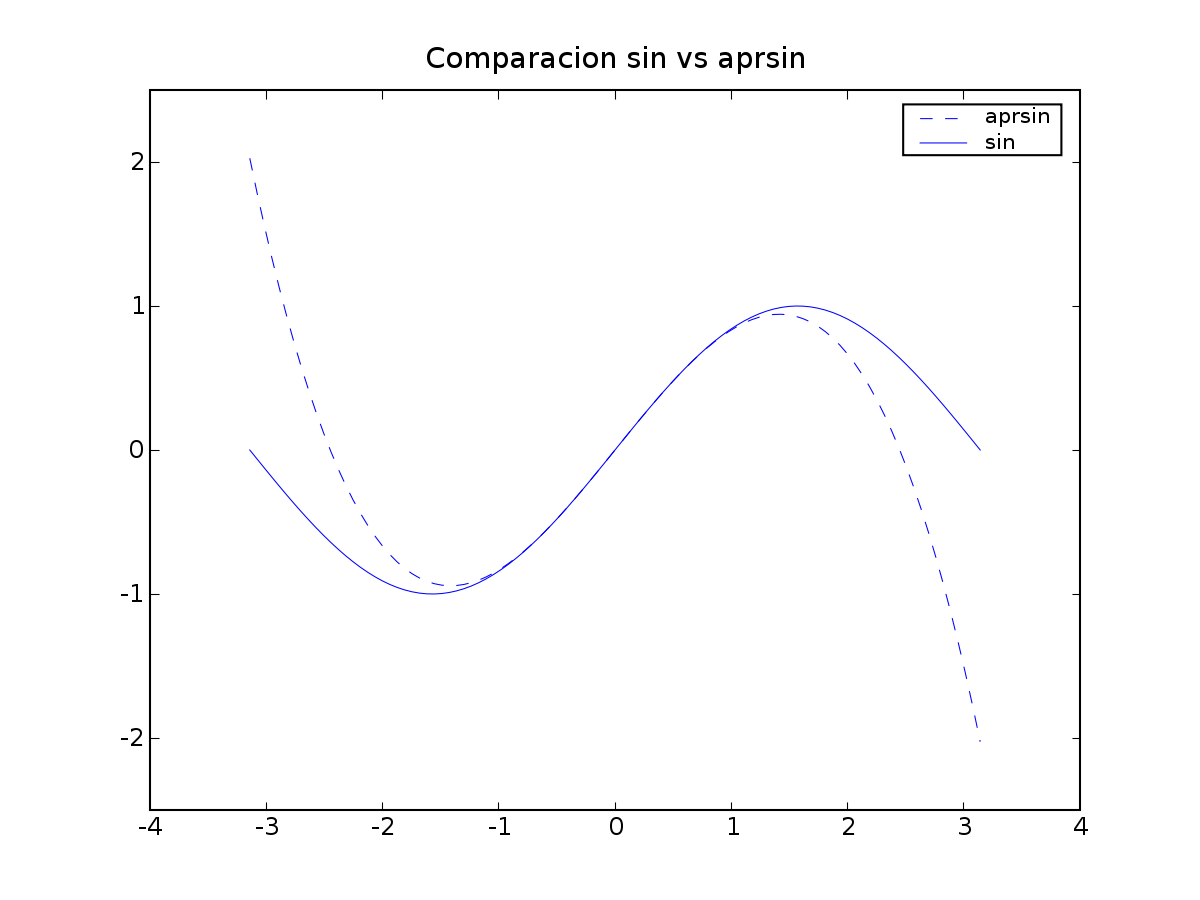
\includegraphics[%
    width=8cm, keepaspectratio]{figuras/figuraejemplo1.png}
  \end{figure}
\end{frame}

\begin{frame}[containsverbatim]
  \frametitle{La funci\'on \texttt{help}} En Matlab casi todo es una
  funci\'on.  Cada una de ellas contiene una peque\~na ayuda para que
  no sea necesario consultar ning\'un manual.  Para consultar la ayuda
  disponemos de la funci\'on \texttt{help}.  Por ejemplo, para saber
  c\'omo utilizar la funci\'on \texttt{eig}:
\begin{verbatim}
>> help eig
\end{verbatim}
\end{frame}

\begin{frame}
  \frametitle{Argumentos}\framesubtitle{Variables y argumentos} En
  cualquier lenguaje de programaci\'on es muy importante separar los
  conceptos de variable y de argumento:
  \begin{description}
  \item[Argumento] Es cualquier elemento manipulable de un c\'odigo.
    En Matlab son los escalares, las matrices, las funciones...
  \item[Variable] Es el contenedor que se usa para manipular
    argumentos.  Su funci\'on principal es darle un nombre.
  \end{description}
\end{frame}

\begin{frame}[containsverbatim]
  \frametitle{Argumentos}\framesubtitle{Matrices} En Matlab el
  concepto de n\'umero se extiende considerablemente.  Los escalares,
  vectores y matrices son completamente equivalentes.
  \begin{normalsize}
\begin{verbatim}
>> a=pi
a = 3.1416
>> a(1)
ans = 3.1416
>> a(1,1)
ans = 3.1416
>> a(1,1,1)
ans = 3.1416
\end{verbatim}
  \end{normalsize}
  En cualquier otro lenguaje esta llamada provocar\'ia un error
\end{frame}

\begin{frame}[containsverbatim]
  \frametitle{Argumentos}\framesubtitle{Matrices (II)} Todos los
  elementos \emph{num\'ericos} de una matriz son reales de doble
  precisi\'on a no ser que forcemos lo contrario.
\begin{verbatim}
>> b=105
b = 105
>> b=105.
b = 105
>> b=1050e-1
b = 105
>> b=1.05e2
b = 105
\end{verbatim}
\end{frame}

\begin{frame}[containsverbatim]
  \frametitle{Argumentos}\framesubtitle{Matrices: crear una matriz} La
  notaci\'on en este caso sirve para diferenciar si los elementos se
  introducen por filas o por columnas.
  \begin{itemize}
  \item El espacio o la coma \texttt{(,)} separan elementos de una
    misma fila.
  \item El retorno de carro, tanto expl\'icito como impl\'icito
    \texttt{;} separan elementos de una misma columna
  \end{itemize}
  \begin{description}
  \item[Ejemplo] Introducir la matriz: $M=\left(
      \begin{array}{lll}
        1 & 2 & 3 \\ 
        4 & 5 & 6 \\ 
        7 & 8 & 9
      \end{array}
    \right)$
  \end{description}
\begin{verbatim}
  >> M = [1,2,3;4,5,6;7,8,9]
\end{verbatim}
\end{frame}

\begin{frame}
  \frametitle{Argumentos}\framesubtitle{Matrices : Ejercicio}
  \begin{description}
  \item[Ejercicio:] Escribir la matriz anterior de otras tres maneras
    distintas
$$
M=\left(
  \begin{array}{lll}
    1 & 2 & 3 \\ 
    4 & 5 & 6 \\ 
    7 & 8 & 9
  \end{array}
\right)
$$
\end{description}

\end{frame}


\begin{frame}[containsverbatim]
  \frametitle{Argumentos}\framesubtitle{Secuencias}
  \begin{description}
  \item [secuencias] Son argumentos dedicados a contar con n\'umeros
    enteros.  Aparecen siempre que necesitemos un contador (bucles,
    intervalos). Su sintaxis es:
  \end{description}
\begin{verbatim}
inicio:salto:final
\end{verbatim}
  \begin{Example}
\begin{verbatim}
>> secuencia = 0:2:10
secuencia =

   0   2   4   6   8  10

\end{verbatim}
  \end{Example}
\end{frame}

\begin{frame}
  \frametitle{Argumentos}\framesubtitle{Submatrices} Supongamos que a
  partir de esta matriz:
$$M=\left( 
\begin{array}{lllll}
  11 & 12 & 13 & 14 & 15\\ 
  21 & 22 & 23 & 24 & 25\\ 
  31 & 32 & 33 & 34 & 35\\ 
  41 & 42 & 43 & 44 & 45\\ 
  51 & 52 & 53 & 54 & 55
\end{array}
\right)
$$
queremos sustraer la siguiente:
$$M=\left( 
\begin{array}{lll}
  33 & 34 & 35\\ 
  43 & 44 & 45\\ 
  53 & 54 & 55
\end{array}
\right)
$$
\end{frame}
\begin{frame}[containsverbatim]
  \frametitle{Argumentos}\framesubtitle{Submatrices (II)} Para denotar
  las filas y columnas que queremos seleccionar usaremos las
  secuencias.  En este caso queremos las filas de la tercera a la
  quinta y las columnas de la tercera a la quinta:
\begin{verbatim}
>> SM = M(3:5,3:5)
\end{verbatim}
  \begin{description}
  \item[Ejercicio:] C\'omo extraer\'iamos la matriz $ M=\left(
      \begin{array}{lll}
        21 & 23 & 25\\ 
        41 & 43 & 45
      \end{array}
    \right) $?
  \end{description}
\end{frame}

\begin{frame}[containsverbatim]
  \frametitle{Argumentos}\framesubtitle{Submatrices (III)}
  \begin{description}
  \item[Soluci\'on:]
  \end{description}
\begin{verbatim}
>> M(2:2:4,1:2:5)
ans =

  21  23  25
  41  43  45
\end{verbatim}
\end{frame}

\begin{frame}
  \frametitle{Argumentos}\framesubtitle{Complejos, texto y variables
    l\'ogicas}
  \begin{description}
  \item[N\'umeros complejos:] El n\'umero imaginario en Matlab se
    trata como otro cualquiera y se simboliza con \texttt{i},
    \texttt{j}, \texttt{I}, o \texttt{J}. Las matrices de complejos se
    tratan igual que las reales.
  \item[Cadenas de texto:] Se introducen entre comillas simples
  \item[Variables l\'ogicas:] Son \texttt{true} y \texttt{false}.  En
    realidad es \texttt{0} para falso y distinto de \texttt{0} para
    verdadero.
  \end{description}
\end{frame}

\begin{frame}[containsverbatim]
  \frametitle{Variables no convencionales}\framesubtitle{Estructuras
    de datos} Sirven para agrupar argumetos de distintos tipos en
  estructuras de tipo \'arbol.  Cada rama se denota por un punto:
  \begin{Example}
\begin{verbatim}
>> ed.num = 1.234;
>> ed.str = 'Hola, Mundo';
>> ed.logic.verdadero = true
ed =
{
  logic =
  {
    verdadero = 1
  }
...
\end{verbatim}
  \end{Example}
\end{frame}

\begin{frame}[containsverbatim]
  \frametitle{Variables no convencionales}\framesubtitle{Celdas o
    \emph{Cell Arrays}} Otra estructura de datos son las celdas.  Son
  parecidas a las matrices con la diferencia que sus elementos pueden
  ser de distintos tipos.  Para introducir una estructura de celdas se
  usan las llaves ( \{ \} ).  Por ejemplo:
  \begin{Example}
\begin{verbatim}
>> celda={1.234,'hola';true,false}
celda =
{
  [1,1] = 1.2340
  [2,1] = 1
  [1,2] = hola
  [2,2] = 0
}
\end{verbatim}
  \end{Example}
\end{frame}

\begin{frame}[containsverbatim]
  \frametitle{Function handles} Los \emph{Function handles} sirven
  para asignar una funci\'on a una variable.  Es el recurso m\'as
  complejo pero a la vez m\'as potente de Matlab. El s\'imbolo de un
  \emph{Function handle} es \texttt{@}
  \begin{Example}
\begin{verbatim}
>> fhsin=@sin
fhsin =

sin

>> fhsin(pi/2)
ans = 1
\end{verbatim}
  \end{Example}
\end{frame}

\begin{frame}
  \frametitle{Function handles}\framesubtitle{Ejercicio in\'util
  pero muy instructivo}
  \begin{description}
  \item[Ejercicio:] Construir una estructura de datos que contenga las
    funciones trigonom\'etricas $\sin$, $\cos$, y $\tan$ y llamarlas
    en el punto $\frac{\pi}{2}$ a partir de la estructura misma.
  \end{description}
\end{frame}

\begin{frame}[containsverbatim]
  \frametitle{Function handles}\framesubtitle{Soluci\'on}
\begin{verbatim}
>> struct={@sin,@cos,@tan};
>> struct{1}(pi/2)
ans = 1
>> struct{2}(pi/2)
ans =  6.1230e-17
>> struct{3}(pi/2)
ans =  1.6332e+16
\end{verbatim}
\end{frame}

\begin{frame}
  \frametitle{Operadores}
  \begin{description}
  \item[{Operadores aritm\'eticos matriciales}] \texttt{+,-,*,/,\^}
  \item[{Operadores aritm\'eticos escalares}] \texttt{.*,./,.\^}
  \item[{Operadores l\'ogicos}] \texttt{\&,|,!}
  \item[{Operadores de comparaci\'on}] \texttt{<,>,==,<=,>=,!=}
  \item[{Operadores de conjuntos l\'ogicos}] \texttt{\&\&,||}
  \end{description}

\end{frame}

\begin{frame}[containsverbatim]
  \frametitle{Cuidado}
Los resultados de operadores matriciales y escalares pueden confundirse
f\'acilmente
\begin{verbatim}
>> a=rand(3,3);b=rand(3,3);
>> a*b
ans =
  0.54816  0.15934  0.56038
  1.46342  0.99260  1.04965
  1.42294  0.89033  1.10239
>> a.*b
ans =
  0.36302  0.03278  0.00889
  0.38461  0.21906  0.85711
  0.37734  0.55768  0.05756
\end{verbatim}
\end{frame}

\begin{frame}[containsverbatim]
   \frametitle{Cuidado}
   O dar lugar a resultados imprevistos, una buena manera de perder toda
la tarde...
\begin{verbatim}
>> a=[1,2,3;4,5,6;7,8,9];
>> a.^pi
ans =
  1.0000    8.8250   31.5443
 77.8802  156.9925  278.3776
451.8079  687.2913  995.0416
>> a^pi
ans =
 694.29 - 0.44i   853.97 - 0.12i  1013.65 + 0.20i
1574.29 - 0.05i  1934.44 - 0.01i  2294.60 + 0.02i
2454.28 + 0.34i  3014.92 + 0.09i  3575.56 - 0.16i
\end{verbatim}
\end{frame}

\begin{frame}
  \frametitle{Cuidado} \framesubtitle{Ejercicio} con \[ A_{ij}=
  \left(\begin{array}{lll}
      1 & 2 & 3\\
      4 & 5 & 6\\
      7 & 8 & 9
    \end{array}\right)
  ,\quad b_i= \left(
    \begin{array}{l}
      1\\
      2\\
      3
    \end{array}
  \right)
  y \quad c_i=(4,5,6)
  \]
  calcular:
  \begin{itemize}
  \item $A \cdot b$
  \item $\sum_i A_{ji} c_i$
  \item $b \cdot c$
  \item $A_ij \cdot (b \cdot c)_{ij}$
  \end{itemize}
  luego aplicar al resultado de cada operaci�n la funci�n $x^2sin(x)$
  
  
\end{frame}

\begin{frame}
  \frametitle{Sentencias y control del flujo de ejecuci\'on}
  \begin{itemize}
  \item Las sentencias son las palabras clave necesarias para
    programar.
  \item Son comunes a la mayor\'ia de los lenguajes.
  \item Implementan tareas b\'asicas como los bucles, los
    condicionales, los casos...
  \end{itemize}
\end{frame}

\begin{frame}[containsverbatim]
  \frametitle{Sentencias} \framesubtitle{Sentencia \texttt{if}} Este
  es un ejemplo de sentencia condicional
  \begin{Example}
\begin{verbatim}
if saludo % saludo==1, saludo==true
  disp('hola')
else
  disp('no te saludo')
end
\end{verbatim}
  \end{Example}
  �Cu�l es la entrada y cu�l es la salida?
\end{frame}

\begin{frame}[containsverbatim]
  \frametitle{Sentencias} \framesubtitle{Sentencia \texttt{for}} Es la
  sentencia utilizada para programar los bucles:
  \begin{Example}
\begin{verbatim}
function primetest(n)
sprintf('Numeros primos de 1 a %i\n',n)
  for i=1:n
    if isprime(i)
      disp(i)
    end
  end
end
\end{verbatim}
  \end{Example}
  �Qu� hace esta subrutina?
\end{frame}

\begin{frame}[containsverbatim]
  \frametitle{Sentencias} \framesubtitle{Sentencia \texttt{switch}}
  \begin{Example}
\begin{verbatim}
function primetest2(n)
  sprintf('�Es primo el numero %i? \n',n)
  primosn = isprime(n);
  switch primosn
    case true
      disp('si')
    case false
      disp('norrrrr')
  end
end
\end{verbatim}
  \end{Example}
  �Qu� hace esta funci\'on?
\end{frame}

\begin{frame}
  \frametitle{Sentencias} \framesubtitle{Otras sentencias}
  \begin{description}
  \item[\texttt{while}] Es un bucle controlado por una condici\'on
    l\'ogica
  \item[\texttt{do-until}] Igual a \texttt{while} pero con la
    condici\'on l\'ogica complementaria
  \item[\texttt{try}] Sentencia de control a prueba de errores
  \item[\texttt{break}] Clave para el control de unidades de programa
  \item[\texttt{continue}] Idem
  \item[\texttt{return}] Devuelve el control al programa principal
  \end{description}
\end{frame}

\begin{frame}[containsverbatim]
  \frametitle{Funciones an\'onimas} Una de las posibilidades de los
  \emph{Function handles} es definir funciones sin necesidad de un
  archivo adicional.  Para ello especificaremos la cabecera y luego
  escribiremos la funci\'on
  \begin{Example}
\begin{verbatim}
>> testfh=@(x,y) exp(-(x.^2+y.^2));
>> testfh(1,i)
ans = 1
\end{verbatim}
  \end{Example}
\end{frame}

\begin{frame}
  \frametitle{conclusiones}
  \begin{itemize}
  \item El lenguaje Matlab es bastante limitado
  \item Es sencillo y tiene una sintaxis clara
  \item Sus estructuras son muy matem�ticas
  \item Est� basado en funciones y a�n no conocemos ninguna.
  \item Sin una biblioteca de funciones Matlab no es NADA
  \end{itemize}
\end{frame}



\section{La biblioteca de funciones}

\subsection{\'Algebra y C\'alculo}

\begin{frame}
  \frametitle{\'Algebra}\framesubtitle{Creaci\'on de matrices} Es muy
  importante utilizar las funciones siguientes para iniciar datos.  A
  partir de ellas se puede crear casi cualquier matriz.
  \begin{description}
  \item[eye] Matriz identidad
  \item[linspace] Vector de elementos separados linealmente
  \item[logspace] Vector de elementos separados exponencialmente
  \item[meshgrid] Matriz equiespaciada de dos dimensiones
  \item[ones] Matriz llena de unos
  \item[zeros] Matriz llena de ceros
  \item[rand] Matriz llena de n\'umeros pseudoaleatorios
  \end{description}
\end{frame}

\begin{frame}
  \frametitle{\'Algebra}\framesubtitle{Manipulaci\'on de matrices} Muy
  importante combinarlas con las anteriores
  \begin{description}
  \item[reshape] Da a la matriz la forma requerida sin cambiar el
    n\'umero de elementos
  \item[transpose] Traspuesta. Equivale a \texttt{.'}
  \item[ctranspose] Traspuesta compleja conjugada.  Equivalente a
    \texttt{'}
  \item[rot90] Gira el bloque de la matriz 90�
  \end{description}
\end{frame}

\begin{frame}[containsverbatim]
  \frametitle{\'Algebra}\framesubtitle{Resoluci\'on de sistemas de
    ecuaciones lineales} Para resolver un sistema de ecuaciones del
  tipo $\vec y =\mathbf{A} \vec x$ s\'olo tenemos que utilizar el
  operador de resoluci\'on de este tipo de ecuaciones.
  \begin{Example}
\begin{verbatim}
>> A=[1,0;2,1];y=[2;4];
>> x=A\y
x =

  2
  0 
\end{verbatim}
  \end{Example}
\end{frame}

\begin{frame}
  \frametitle{C\'alculo} \framesubtitle{C\'alculo simb\'olico} Tanto
  Matlab como Octave tienen soporte para variables simb\'olicas con el
  atributo \texttt{sym}
  pero no son int\'erpretes especializados.\\
  Algunos programas especializados en c\'alculo simb\'olico son
  Maple,Mupad y Maxima.
\end{frame}

\begin{frame}
  \frametitle{C\'alculo} \framesubtitle{Polinomios} Matlab opera
  polinomios almacenando sus coeficientes como un vector.
  \begin{Example}
    El polinomio $p=x^2+x$ es \texttt{[1 1 0]}
  \end{Example}
  \begin{description}
  \item[poly] Obtiene el polinomio caracter\'istico de una matriz
  \item[roots] Obtiene las ra\'ices de un polinomio
  \item[polyval] Devuelve el valor de un polinomio en el punto dado
  \item[polyder] Deriva un polinomio
  \item[polyint] Integra un polinomio
  \end{description}

\end{frame}

\begin{frame}
  \frametitle{C\'alculo}\framesubtitle{Integraci\'on num\'erica}
  \begin{description}
  \item[{quad quadl}] Integraci\'on num\'erica de una funci\'on o de
    una funci\'on an\'onima
  \item[dblquad] Calcula una integral doble.  En Octave se llaman
    \texttt{quad2dc} y \texttt{quad2dg} dependiendo del algoritmo.
  \item[triplequad] Integral triple
  \item[trapz] Integra por la regla del trapecio una serie discreta de
    puntos
  \end{description}
\end{frame}

\begin{frame}
  \frametitle{C\'alculo}\framesubtitle{Ejercicio} Hacer la integral
$$ I=\int_{-\infty}^{\infty}\int_{-\infty}^{\infty}e^{-(x^2+y^2)}dx\ dy
$$
de soluci\'on $\pi$ con un \'unico comando
\begin{description}
\item[Pista] Utilizar una funci\'on an\'onima
\item[Pista] Por problemas de precisi\'on num\'erica hay que integrar
  de -10 a 10.
\end{description}
\end{frame}

\begin{frame}[containsverbatim]
  \frametitle{C\'alculo}\framesubtitle{Soluci\'on}
  \begin{itemize}
  \item Matlab
  \end{itemize}
\begin{verbatim}
>> dblquad(@(x,y) exp(-(x.^2+y.^2)),-10,10,-10,10)
ans = 3.1416
\end{verbatim}
  \begin{itemize}
  \item Octave
  \end{itemize}
\begin{verbatim}
>> quad2dg(@(x,y) exp(-(x.^2+y.^2)),-10,10,-10,10)
ans = 3.1416
\end{verbatim}
\end{frame}

\subsection{Gr\'aficos}

\begin{frame}
  \frametitle{Introducci\'on}
  \begin{itemize}
  \item Representar datos gr\'aficamente en Matlab es muy sencillo e
    intuitivo
  \item Las funciones son pocas porque no hay demasiadas necesidades
  \item Matlab incluye un visualizador (Explorador de datos) que no
    veremos
  \item No hay que dejarse encandilar por las posibilidades en
    representaci\'on gr\'afica.  Una curva bien pensada es mucho mejor
    que una superficie.
  \item \textbf{S\'olo veremos curvas en el plano, el resto no tiene
      ning\'un misterio}
  \end{itemize}
\end{frame}

\begin{frame}[containsverbatim]
  \frametitle{Plot} La manera m\'as f\'acil de representar datos es
  mediante el comando \texttt{plot}.
  \begin{Example}
    Representar una curva en el plano a partir de dos series de datos
\begin{verbatim}
      >> x=linspace(0,500,100000);
      >> plot(x,exp(-x/100).*sin(x))
\end{verbatim}
  \end{Example}
  Para dibujar la funci\'on $e^{-\frac{x}{100}}\sin x$ con $x \in
  [0,500]$
\end{frame}


\begin{frame}
  \frametitle{Plot}
  \begin{figure}[h]
    \centering{}
    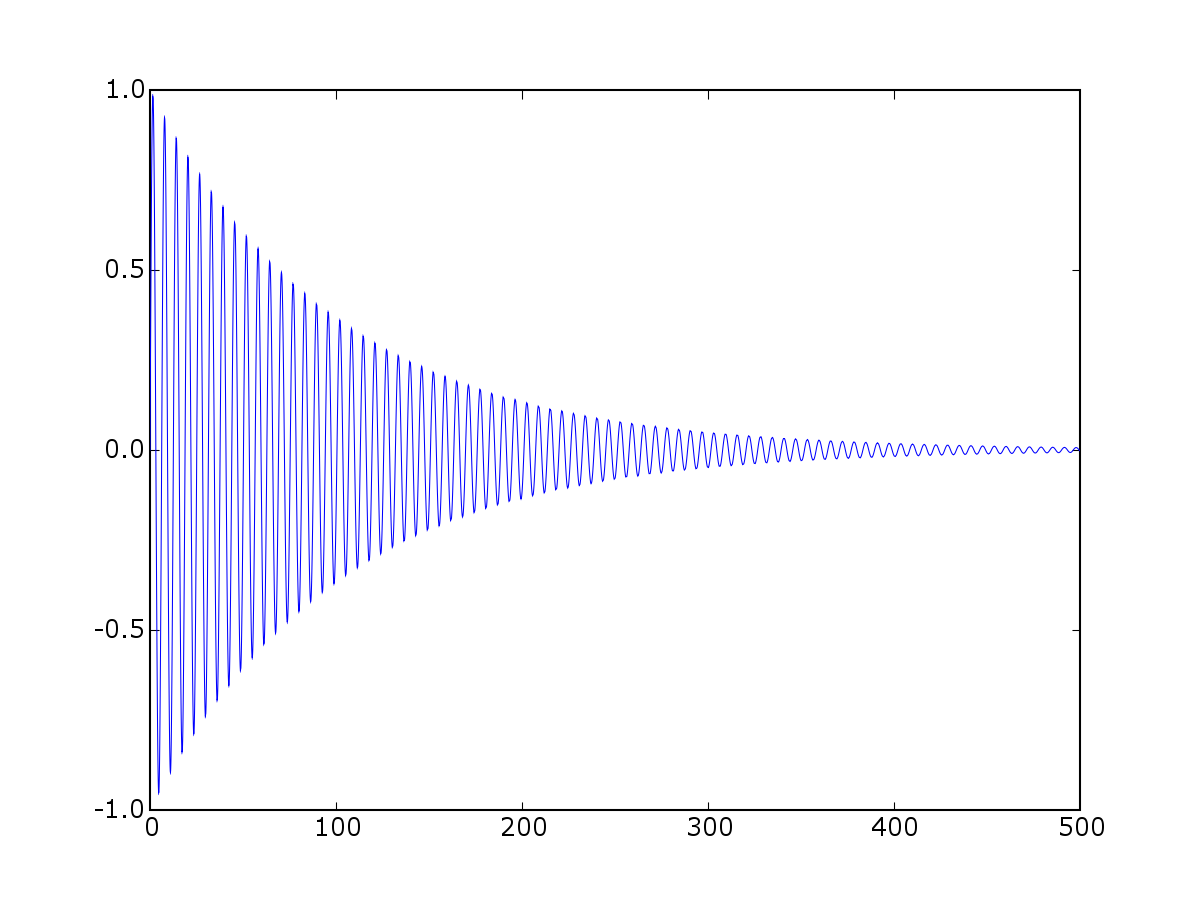
\includegraphics[%
    width=9cm, keepaspectratio]{figuras/simpleplot.png}
  \end{figure}
\end{frame}

\begin{frame}[containsverbatim]
  \frametitle{Plot} Los atributos de las gr�ficas se introducen con la
  ventana activa
  \begin{Example}
\begin{verbatim}
>> title('Una funcion cualquiera')
>> xlabel('Tiempo')
>> ylabel('Amplitud')
\end{verbatim}
  \end{Example}
\end{frame}


\begin{frame}
  \frametitle{Plot}
  \begin{figure}[h]
    \centering{}
    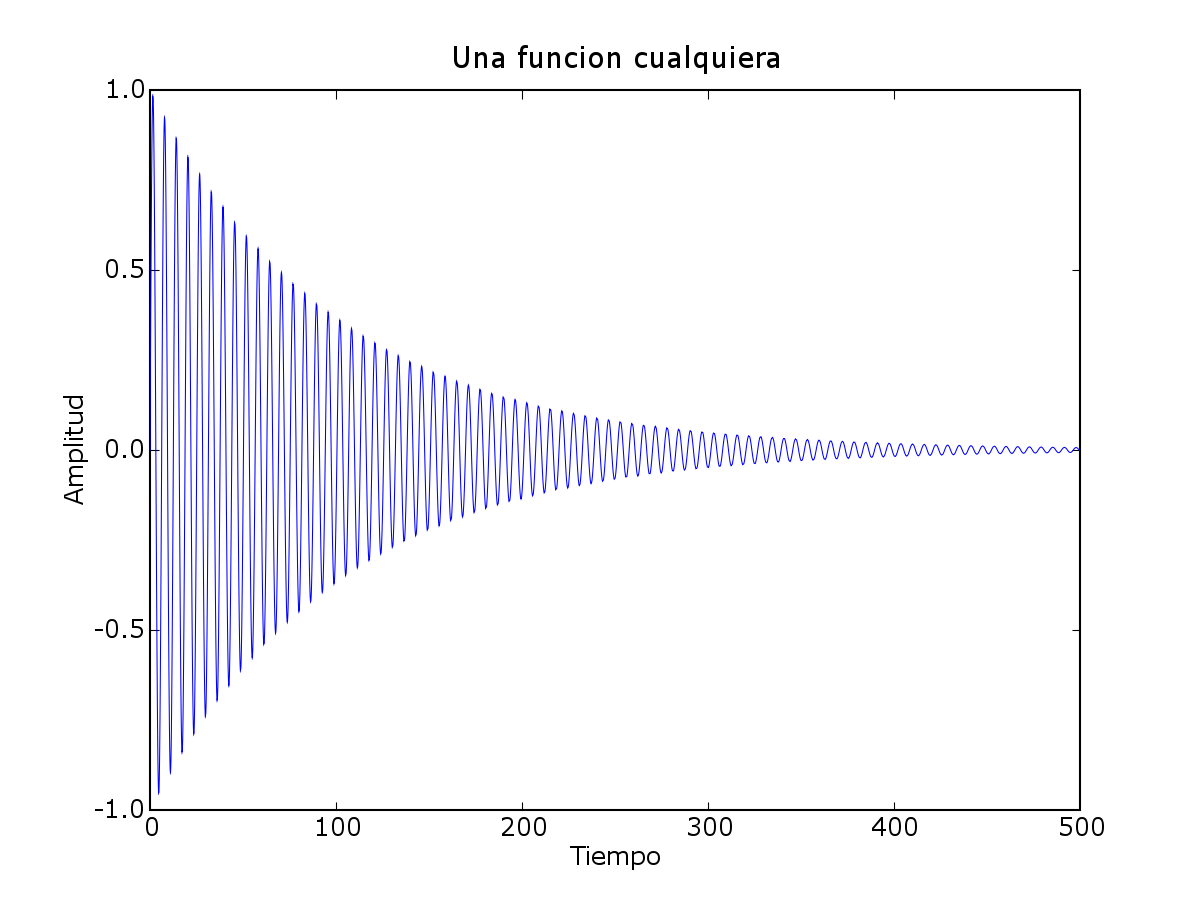
\includegraphics[%
    width=9cm, keepaspectratio]{figuras/titleplot.png}
  \end{figure}
\end{frame}

\begin{frame}[containsverbatim]
  \frametitle{Plot} Dentro del mismo comando podemos poner varias
  curvas con distintos estilos
  \begin{Example}
\begin{verbatim}
>> x=linspace(-pi,pi,100);
>> plot(x,sin(x),'m:',...
     x,cos(x),'k^',x,tan(x),'bx')
>> axis([-pi,pi,-2,2])
>> grid on
>> legend('linea de puntos magenta',...
          'triangulos negros',...
          'cruces azules')
\end{verbatim}
  \end{Example}
\end{frame}

\begin{frame}
  \frametitle{Plot}
  \begin{figure}[h]
    \centering{}
    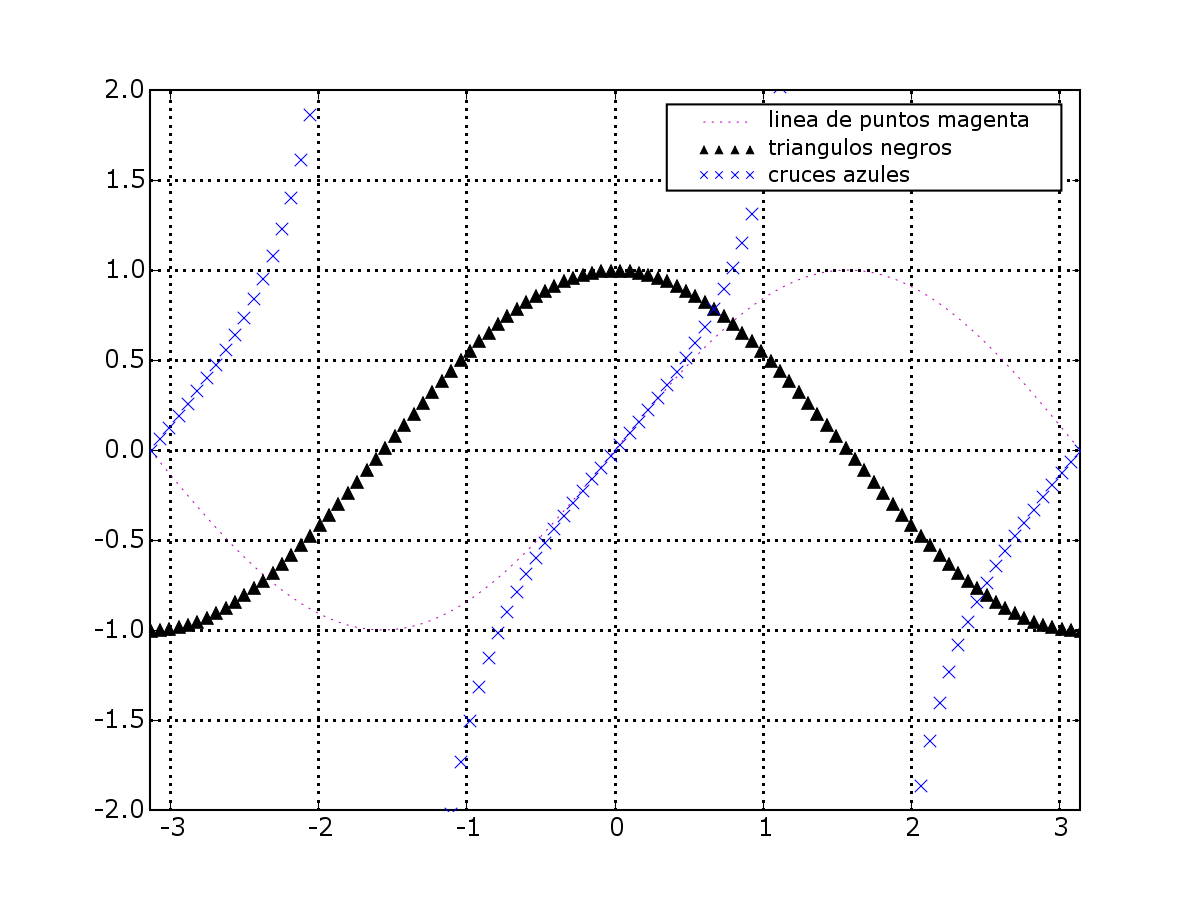
\includegraphics[%
    width=9cm, keepaspectratio]{figuras/legendplot.png}
  \end{figure}
\end{frame}

\begin{frame}
  \frametitle{Plot}
  \begin{itemize}
  \item La ventana gr�fica se borra autom�ticamente cada vez que
    dibujamos algo %\pause
  \item Para cambiar el comportamiento anterior se usa la funci\'on
    \texttt{hold} %\pause
  \item \texttt{hold on} mantiene todo lo dibujado en la pantalla
    % \pause
  \item \texttt{hold off} devuelve el comportamiento inicial.
  \end{itemize}
\end{frame}

\begin{frame}
  \frametitle{Plot}
  \begin{itemize}
  \item Las ventanas gr�ficas se manipulan con la funci\'on
    \texttt{figure} %\pause
  \item \texttt{figure} se llama con un n\'umero que es el n\'umero de
    la ventana %\pause
  \item Si utilizamos un n\'umero que no existe creamos una ventana
    % \pause
  \item Si utilizamos un n\'umero existente activaremos la ventana
  \end{itemize}
\end{frame}

\begin{frame}[containsverbatim]
  \frametitle{Subplot} Subplot es el comando que permite poner m\'as
  de una figura en una ventana.  Su uso es parecido al de combinar
  \texttt{figure} y \texttt{plot}
  \begin{Example}
\begin{verbatim}
>> x=linspace(-pi,pi,100);
>> subplot(2,2,1)
>> plot(x,sin(x))
\end{verbatim}
    De este modo generamos la primera de las subfiguras en el primero
    de los cuatro sectores.
  \end{Example}
\end{frame}

\begin{frame}
  \frametitle{Subplot}
  \begin{figure}[h]
    \centering{}
    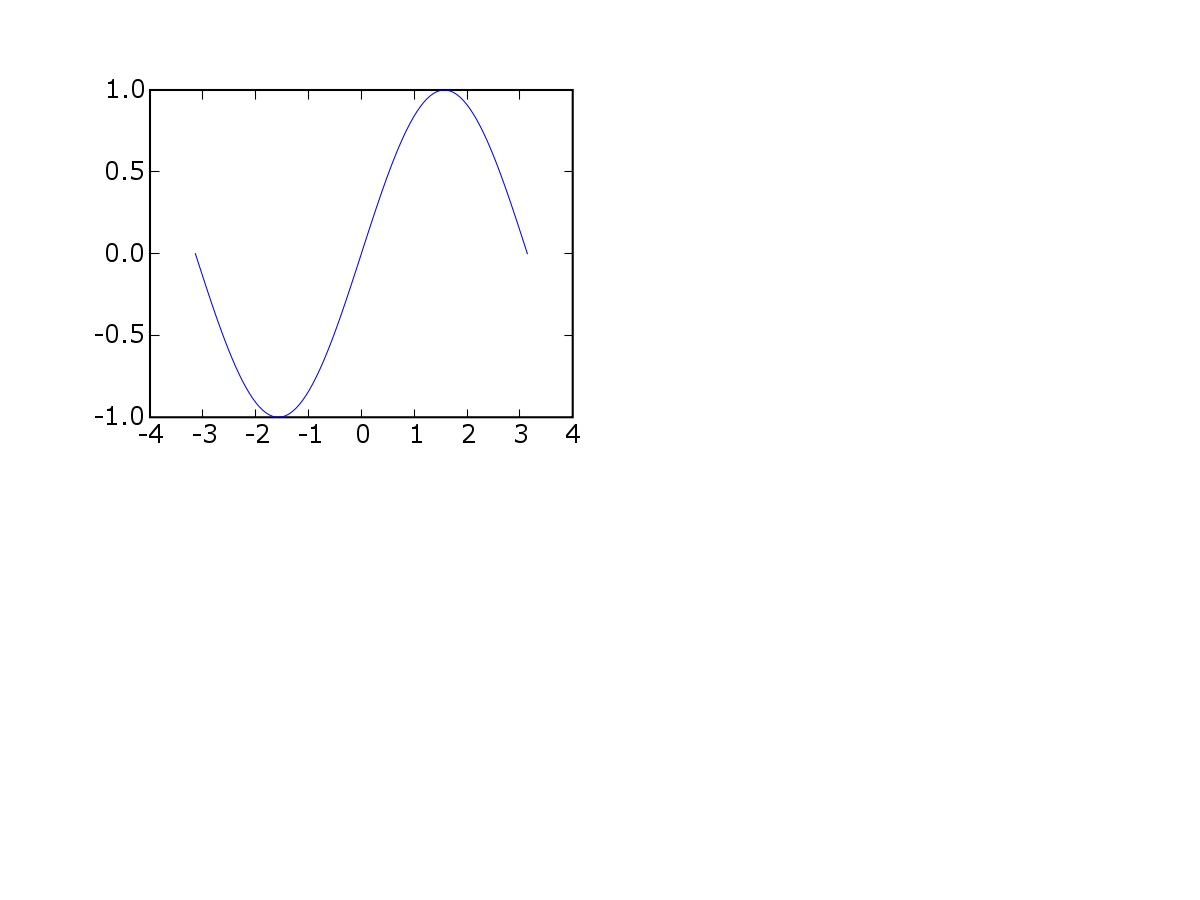
\includegraphics[%
    width=9cm, keepaspectratio]{figuras/subplot1.png}
  \end{figure}
\end{frame}

\begin{frame}[containsverbatim]
  \frametitle{Subplot} Ahora completamos los cuatro cuadrantes
  \begin{Example}
\begin{verbatim}
>> subplot(2,2,2)
>> plot(x,cos(x))
>> subplot(2,2,3)
>> plot(x,sinh(x))
>> subplot(2,2,4)
>> plot(x,cosh(x))
\end{verbatim}
  \end{Example}
\end{frame}

\begin{frame}
  \frametitle{Subplot}
  \begin{figure}[h]
    \centering{}
    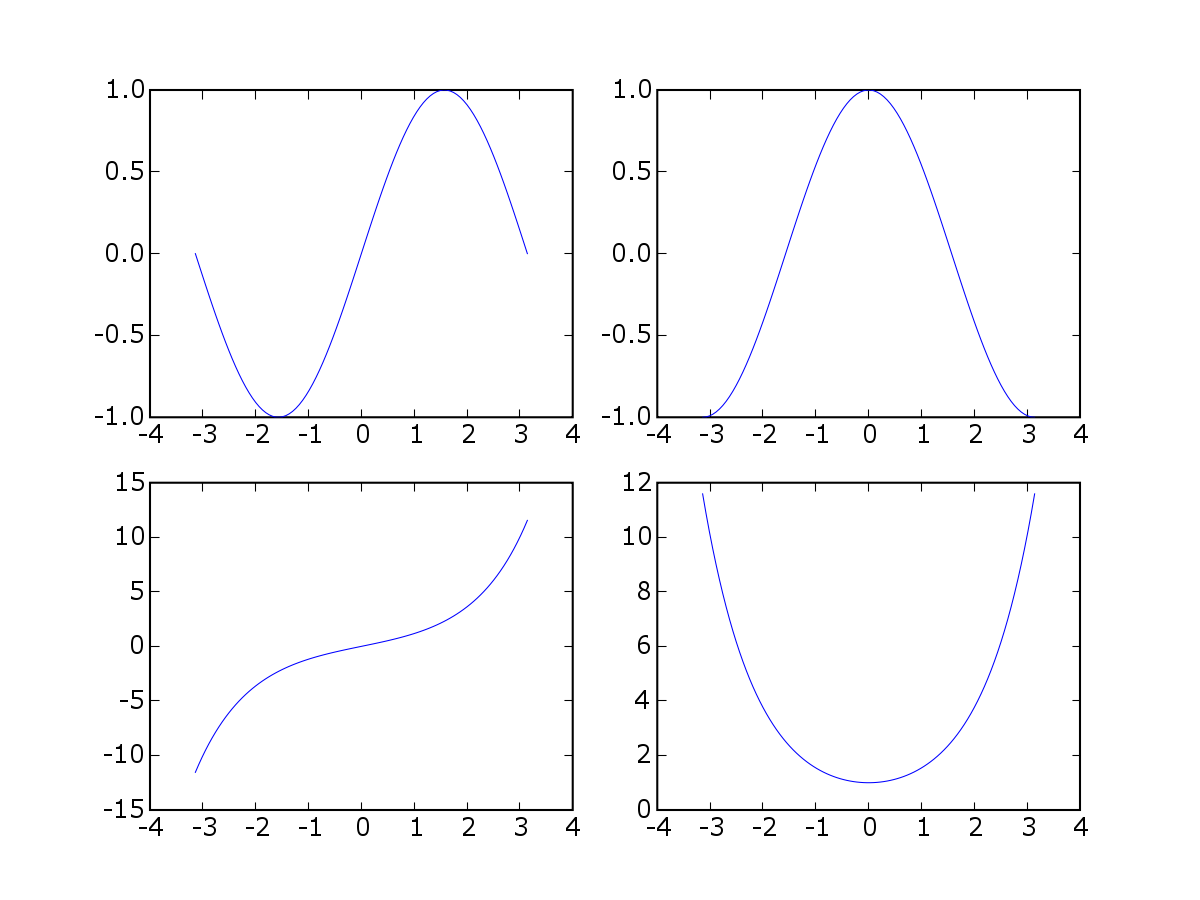
\includegraphics[%
    width=9cm, keepaspectratio]{figuras/subplot2.png}
  \end{figure}
\end{frame}

\begin{frame}
  \frametitle{\texttt{semilogx}, \texttt{semilogy} y \texttt{loglog}}
  \begin{description}
  \item[semilogx] Dibuja una curva con el eje \texttt{x} en escala
    logar\'itmica
  \item[semilogy] Dibuja una curva con el eje \texttt{y} en escala
    logar\'itmica
  \item[loglog] Dibuja una curva con ambos ejes en escala
    logar\'itmica
  \end{description}
\end{frame}

\begin{frame}
  \frametitle{Ejercicio} Representar en una misma ventana y dos frames
  (uno superior y otro inferior) la funci\'on:
$$\sqrt{x}\ \sin(\frac{1}{x}) \qquad x \in [0.001,1]
$$
en escala normal y en escala semilogar\'itmica en el eje \texttt{x}
\end{frame}

\begin{frame}[containsverbatim]
  \frametitle{Ejercicio}
\begin{verbatim}
x=linspace(0.001,1,10000);
subplot(2,1,1)
plot(x,sqrt(x).*sin(1./x))
subplot(2,1,2)
semilogx(x,sqrt(x).*sin(1./x))
\end{verbatim}
\end{frame}

\begin{frame}
  \frametitle{Ejercicio}
  \begin{figure}[h]
    \centering{}
    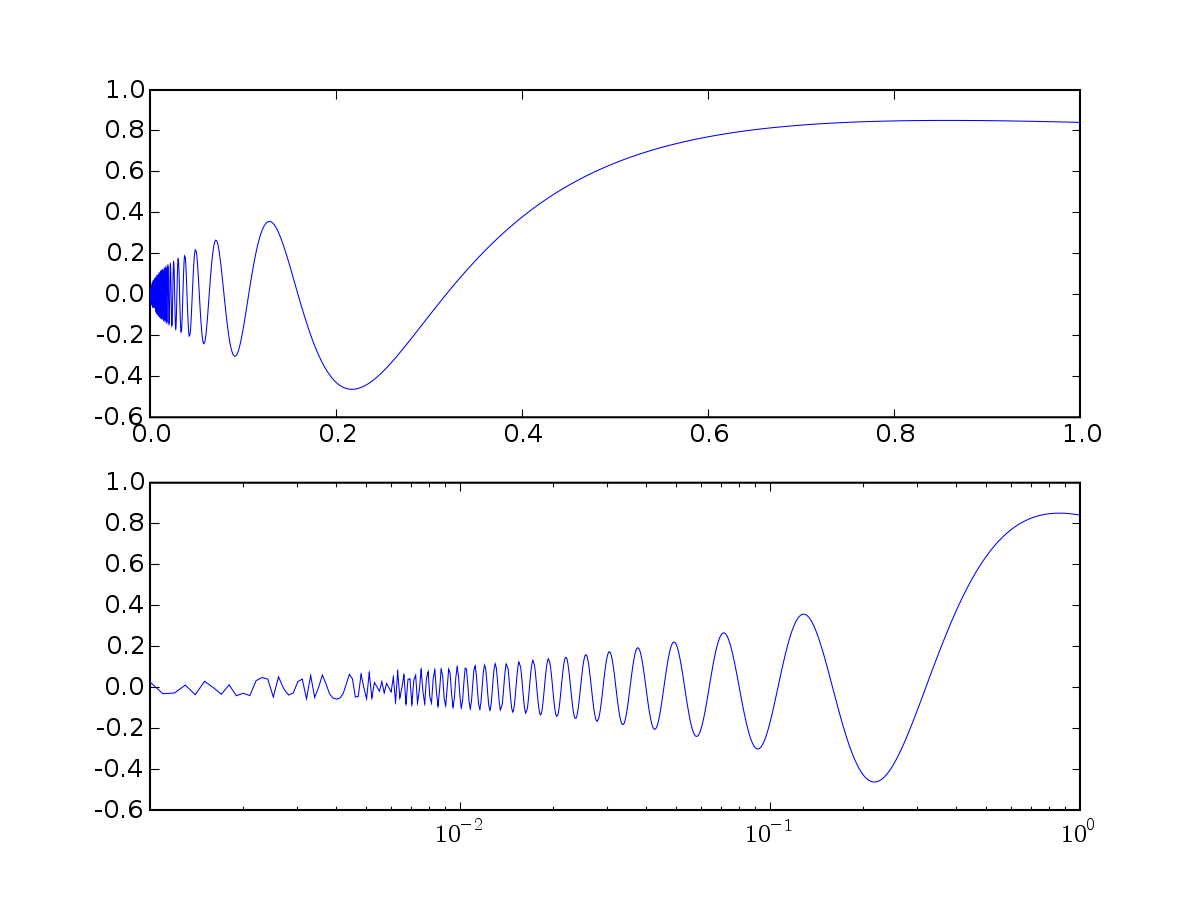
\includegraphics[%
    width=9cm, keepaspectratio]{figuras/ejercicio.png}
  \end{figure}
\end{frame}

\begin{frame}[containsverbatim]
  \frametitle{Contour} La mejor manera de representar superf\'icies en
  tres dimensiones es representar su proyecci\'on en el plano mediante
  isol\'ineas.  La ventaja de esta representaci\'on es que permite
  conocer el valor de la funci\'on con mucha m\'as precisi\'on.
  Probad lo siguiente:
  \begin{Example}
\begin{verbatim}
>> contour(peaks)
\end{verbatim}
  \end{Example}
\end{frame}

\subsection{Toolkits}
\begin{frame}
  \frametitle{An\'alisis de datos}
  \begin{description}
  \item[interp1] Interpolaci\'on sobre una serie de puntos
  \item[interp2] Interpolaci\'on sobre una nube bidimensinal de puntos
  \item[polyfit] Coeficientes del polinomio de grado n que resuelve el
    problema de m\'inimos cuadrados
  \item[fft] Realiza la transformada r\'apida de Fourier de una serie
    de datos.
  \end{description}
\end{frame}

\begin{frame}[containsverbatim]
  \frametitle{\texttt{interp1}}
  \begin{Example}
\begin{verbatim}
>> x=[1 2 3 4 5 6 7 8];
>> y=[1 4 2 5 7 4 2 7];
>> interp1(x,y,7.234,'spline')
ans = 2.3437
>> test=@(x,y,z) interp1(x,y,z,'spline');
>> test(x,y,7.234)
ans = 2.3437
\end{verbatim}
  \end{Example}
\end{frame}

\begin{frame}[containsverbatim]
  \frametitle{\texttt{polyfit}}
  \begin{Example}
\begin{verbatim}
>> x=[1 2 3 4 5 6 7 8];                               
>> y=[2 4 3 5 6 5 7 9];                               
>> coeff=polyfit(x,y,3);                              
>> plot(x,y,'k+',1:0.1:8,...                               
polyval(coeff,1:0.1:8),'b-')
\end{verbatim}
  \end{Example}
\end{frame}

\begin{frame}
  \frametitle{\texttt{polyfit}}
  \begin{figure}[h]
    \centering{}
    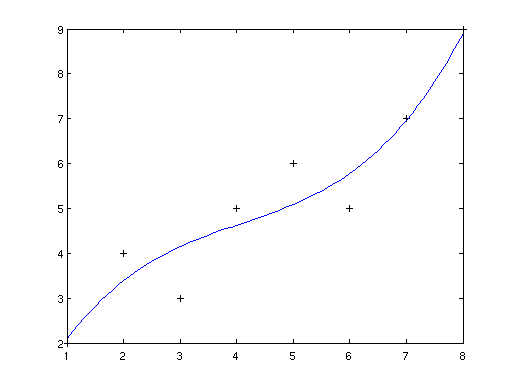
\includegraphics[%
    width=9cm, keepaspectratio]{figuras/testpoly.png}
  \end{figure}
\end{frame}

\begin{frame}
  \frametitle{Estad\'istica descriptiva}
  \begin{description}
  \item[mean] Calcula la media
  \item[std] Calcula la varianza
  \item[median] Calcula la mediana
  \item[sort] Ordena los elementos de menor a mayor
  \item[center] Elimina la media de la muestra
  \end{description}
\end{frame}

\begin{frame}
  \frametitle{EDOs}
  \begin{itemize}
  \item Es probablemente una de las aplicaciones m\'as importantes del
    c\'alculo num\'erico.
  \item Los problemas m\'as comunes son los problemas de Cauchy o de
    evoluci\'on temporal
  \item En el caso de ecuaciones no lineales la soluci\'on num\'erica
    es esencial.  Puede ser que la soluci\'on anal\'itica no se pueda
    hallar (Navier-Stokes)
  \item Lo m\'as importante es saber si nuestro problema es Stiff
  \end{itemize}
\end{frame}

\begin{frame}
  \frametitle{EDOs} \framesubtitle{Diferencias entre Matlab y Octave}
  \begin{itemize}
  \item En este caso Matlab y Octave toman filosof\'ias completamente
    distintas.
  \item Matlab opta por muchas funciones con pocas opciones
  \item Octave opta por una \'unica funci\'on con muchas opciones
  \item Matlab utiliza sus propios algoritmos
  \item Octave utiliza el \texttt{lsode} de ODEPACK
  \end{itemize}
  Como esta introducci\'on es muy breve y casi todos vais a piratear
  Matlab hablaremos s\'olo de Matlab
\end{frame}

\begin{frame}
  \frametitle{EDOs}\framesubtitle{Problemas \emph{stiff}}
  \begin{itemize}
  \item Se dice que un problema es \emph{stiff} cuando el paso
    temporal de integraci\'on viene determinado por la estabilidad y
    no por la precisi\'on. %\pause
  \item Suelen relacionarse con funciones que introducen gradientes
    fuertes o con condiciones de contorno muy restrictivas %\pause
  \item Tambi\'en suelen asociarse a problemas no lineales %\pause
  \item Requieren un esquema de integraci\'on impl\'icito
  \end{itemize}
\end{frame}

\begin{frame}
  \frametitle{EDOs} \subtitle{funciones disponibles}
  \begin{description}
  \item[ode45] Es un esquema Runge-Kutta de cuarto orden y paso
    variable.  Debe ser la primera opci\'on.
  \item[ode113] Esquema Adams (multipaso).
  \item[ode23s] Esquema impl\'icito para problemas \emph{stiff}
  \end{description}
  \begin{itemize}
  \item Hay m\'as funciones de integraci\'on de EDOs pero con estas
    tres es suficiente.
  \item Octave tambi\'en dispone de ellas pero son mucho m\'as lentas
  \item Las funciones terminadas en \emph{s} son para problemas
    \emph{stiff}
  \end{itemize}
\end{frame}

\begin{frame}
  \frametitle{EDOs} \framesubtitle{Ejemplo: la ecuaci\'on de Van der
    Pol} La ecuaci\'on de Van der Pol es:
$$mx^{\prime \prime} - \alpha x^\prime + \beta {x^\prime}^3 +
kx = 0$$ Es una masa oscilante con amortiguamiento lineal y forzado no
lineal.  Adimensionalzando:
$$x^{\prime \prime} +x+\mu ({x^{\prime}}^2-1)x^\prime = 0$$
Matlab ya tiene esta funci\'on en su biblioteca en los casos $\mu=1$
(\texttt{vdp1}) y $\mu=1000$ (\texttt{vdp1000}).  El primero es normal
y el segundo es \emph{stiff}.
\end{frame}

\begin{frame}[containsverbatim]
  \frametitle{EDOs} \framesubtitle{Ejemplo: la ecuaci\'on de Van der
    Pol} Para resolver el problema no \emph{stiff} utilizamos un
  esquema Runge-Kutta, \texttt{ode45}
  \begin{Example}
\begin{verbatim}
  >> [tout,xout]=ode45(@vdp1,[0 20],[2 0])
  >> plot(tout,xout(:,1))
\end{verbatim}
  \end{Example}
\end{frame}

\begin{frame}
  \frametitle{EDOs}\framesubtitle{Soluci\'on del problema no stiff}
  \begin{figure}[h]
    \centering{}
    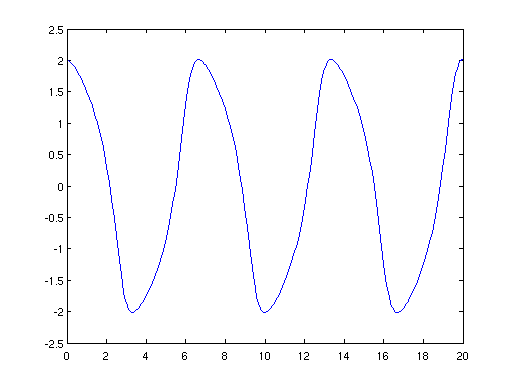
\includegraphics[%
    width=9cm, keepaspectratio]{figuras/vdp1.png}
  \end{figure}
\end{frame}

\begin{frame}[containsverbatim]
  \frametitle{EDOs}\framesubtitle{Ejemplo: la ecuaci\'on de Van der
    Pol}
  \begin{itemize}
  \item Si ahora intentamos resolver el problema para $\mu=1000$ nos
    encontramos con la desagradable sorpresa de que no termina nunca.
  \item Esto es porque el problema es stiff.  Para resolverlo
    cambiamos el m\'etodo de integraci\'on a uno impl\'icito:
  \end{itemize}

  \begin{Example}
\begin{verbatim}
>> [tout,xout]=ode23s(@vdp1000,[0 3500],[2 0]);
>> plot(tout,xout(:,1))
\end{verbatim}
  \end{Example}
\end{frame}

\begin{frame}
  \frametitle{EDOs}\framesubtitle{Soluci\'on del problema stiff}
  \begin{figure}[h]
    \centering{}
    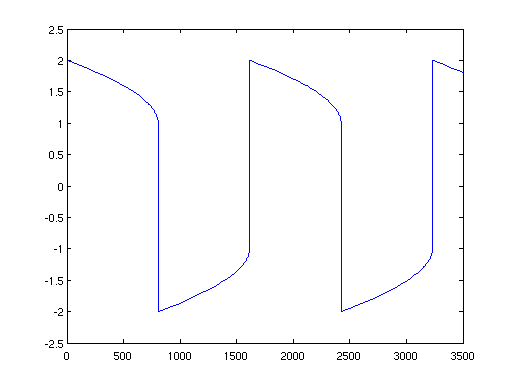
\includegraphics[%
    width=9cm, keepaspectratio]{figuras/vdp1000.png}
  \end{figure}
\end{frame}

\begin{frame}
  \frametitle{Ejercicio}\framesubtitle{Resolver el siguiente problema
    no stiff}
  $$
  \begin{array}{l}
    \dot{x}=a(y-x)\\
    \dot{y}=x(b-z)-y\\
    \dot{z}=xy-cz
  \end{array}\qquad con \qquad 
  a=10,\,\, b=28,\,\, c=\frac{8}{3}$$ con $t \in [0,50]$ y
  $(x_0,y_0,z_0)=(1,1,1)$ mediante la funci�n \texttt{ode45} y
  representarla con \texttt{plot3} como una curva param�trica
  $[x(t),y(t),z(t)]$
\end{frame}

\section{Estilo de programaci\'on}

\subsection{Los 10 mandamientos}

\begin{frame}
  \frametitle{Los 10 mandamientos de Matlab}\framesubtitle{Tabla
    primera}
  \begin{enumerate}
  \item[1] Utilizar los \emph{Function handles} siempre que se pueda.
    % \pause
  \item[2] Usar bucles \texttt{for} s\'olo si es imprescindible.
    % \pause
  \item[3] Utilizar estructuras \texttt{if} planas.  %\pause
  \item[4] Utilizar las funciones de creaci\'on de matrices.  %\pause
  \item[5] Definir las variables de las cabeceras \emph{in situ}.
  \end{enumerate}
\end{frame}

\begin{frame}
  \frametitle{Los 10 mandamientos de Matlab}\framesubtitle{Tabla
    segunda}
  \begin{enumerate}
  \item[6] Utilizar submatrices siempre que se pueda.  %\pause
  \item[7] Tabular bien las estructuras de c\'odigo.  %\pause
  \item[8] Comentar cualquier operaci\'on que lo precise.  %\pause
  \item[9] Escribir cabeceras de ayuda para las funciones.  %\pause
  \item[10] Usar Octave y colaborar en el proyecto.
  \end{enumerate}
\end{frame}

\subsection{Velocidad de ejecuci\'on}
\begin{frame}
  \frametitle{Matlab vs Fortran}
  \begin{itemize}
  \item Matlab no compite con Fortran, son lenguajes distintos para
    objetivos distintos
  \item Matlab es un lenguaje de RAD y prototipado mientras que
    Fortran es ideal para aplicaciones de alto coste computacional.
  \item Ambos lenguajes se complementan perfectamente: las tareas no
    muy exigentes pueden dejarse en Matlab.
  \item Hay que analizar la relaci\'on coste de programaci\'on /
    ganancia de velocidad.
  \end{itemize}
\end{frame}

\begin{frame}
  \frametitle{Matlab vs Fortran (II)} En lo que respecta al estilo de
  programaci\'on ambos tienen una diferencia esencial:
  \begin{itemize}
  \item En Fortran, la velocidad de c\'odigo bien y mal escrito es
    similar
  \item En Matlab, la diferencia de velocidad seg\'un el estilo de
    programaci\'on puede llegar a ser de dos \'ordenes de magnitud.
  \end{itemize}
  Si conseguimos exprimir al m\'aximo Matlab es probable que podamos
  dejar la mayor parte del programa en Matlab y escribir s\'olo
  algunas funciones en C++ o Fortran.
\end{frame}

\begin{frame}[containsverbatim]
  \frametitle{bucles vs notaci\'on matricial} La diferencia de
  velocidad puede ser considerable en c\'alculos similares:
  \begin{Example}
    Sumamos los elementos de dos matrices de 66x66
\begin{verbatim}
a=rand(66) #matriz de 66 x 66 
b=rand(66) 
>> tic;for i=1:66;for j=1:66
c(i,j)=a(i,j)+b(i,j);
end;end;toc 
ans = 0.70488
\end{verbatim}
  \end{Example}
\end{frame}

\begin{frame}[containsverbatim]
  \frametitle{bucles vs notaci\'on matricial} Utilizar la notaci\'on
  matricial suele ser m\'as r\'apido, sencillo y le\'ible que el
  m\'etodo anterior:
  \begin{Example}
\begin{verbatim}
>> tic;c=a.+b;toc 
ans = 0.0022700
\end{verbatim}
  \end{Example}
  Y con $\frac{1}{300}$ veces el tiempo de ejecuci\'on!  Este tiempo
  es parecido al obtenido con C++.
\end{frame}

\begin{frame}
  \frametitle{Y para acabar...}
  \begin{itemize}
  \item Estas transparencias no hubieran sido posibles sin \LaTeX\ y
    Beamer
  \item Recordad que en caso de duda podeis contactar conmigo en:
  \end{itemize}
  \begin{center}
    \texttt{guillemborrell@gmail.com}\\
    \texttt{guillem@torroja.dmt.upm.es}
  \end{center}
\end{frame}

\begin{frame}
  \begin{center}
    \begin{Huge}
      Muchas gracias
    \end{Huge}
  \end{center}
\end{frame}

\end{document}


